\documentclass[journal]{IEEEtran}
\usepackage{amsmath,amssymb,amsfonts}
\usepackage{graphicx}
\usepackage{booktabs}
\usepackage{array}
\usepackage{tikz}
\usepackage{hyperref}

\begin{document}

\title{Sub-50ms Autonomous Physical-Layer Remediation and Millimeter-Scale Fault Localization in Optical Networks Using Hybrid 1D-CNN/Transformer Models on 12-Bit Telemetry}

\author{Salim~Bassam~Assil,~\IEEEmembership{Lead~Systems~Architect,} Batoul~Mowafak~Zain~Alabdin, and~Ahmad~Jalal~B.~Al~Assil%
\thanks{Manuscript received October 2026. This work was supported by CableHunt Networks Ltd. (UK Company Registration No. 16093071) under the Birmingham Optical Testbed and Sovereign Edge AI Initiative.}%
\thanks{S.~B.~Assil, B.~M.~Zain~Alabdin, and A.~J.~B.~Al~Assil are with the Optical Systems and Edge AI Research Group, CableHunt Networks Ltd., 70 Colombo Street, London, SE1 8EE, United Kingdom, and the Birmingham Optical Testbed, West Midlands, United Kingdom (e-mail: assilno1@gmail.com; saleem@cablehunt.co.uk; sassil@psa.ac.ae).}}

\markboth{IEEE/OPTICA JOURNAL OF OPTICAL COMMUNICATIONS AND NETWORKING, VOL.~18, NO.~10, OCTOBER 2026}%
{Assil \MakeLowercase{\textit{et al.}}: Sub-50ms Autonomous Physical-Layer Remediation in Optical Networks}

\maketitle

\begin{abstract}
Passive optical networks (PONs) and dense wavelength-division multiplexed (DWDM) metro trunks suffer from both abrupt hard failures and progressive soft physical-layer degradations. Conventional network management systems rely on coarse 8-bit optical time-domain reflectometry (OTDR) or delayed digital diagnostic monitoring (DDM) polling, resulting in prolonged mean-time-to-repair (MTTR) and undetected pre-failure optical transients. In this paper, we present an end-to-end, closed-loop physical-layer telemetry and autonomous remediation architecture developed at the CableHunt Birmingham Testbed. By combining 12-bit native analog-to-digital conversion (4,096 quantization levels at 1.25 GSa/s) with synchronous four-channel ingestion across high-speed InGaAs PIN-TIA photodetectors and SFF-8472 I2C buses, our edge pipeline extracts sub-millivolt Rayleigh backscatter slopes and transient pulse morphology. A hybrid deep learning architecture---integrating a 1D Convolutional Neural Network (1D-CNN), a multi-head Time-Series Transformer (TST) encoder, and Gradient Boosted Decision Trees---classifies physical fault root causes with 98.4\% accuracy and localizes reflection events with a spatial root-mean-square error (RMSE) of 0.015 m (1.5 cm) and an event dead zone (EDZ) below 0.8 m. Upon detecting anomalous degradation, the engine executes an automated Netmiko/SSH control loop on industrial switches (Cisco IE-3000-8FM), completing dynamic optical power adaptation and wavelength protection switching within 41.8 ms.
\end{abstract}

\begin{IEEEkeywords}
Optical time-domain reflectometry (OTDR), 12-bit ADC telemetry, autonomous network remediation, 1D-CNN, Time-Series Transformer, SFF-8472 DDM, soft failure detection, ITU-T G.652.D.
\end{IEEEkeywords}

\section{Introduction}
\IEEEPARstart{O}{ptical} transport infrastructures form the physical backbone of modern cloud data centers, 5G/6G front-haul links, and national Fiber-to-the-Premises (FTTP) access networks. Despite the massive bandwidth capacity of single-mode optical fibers (ITU-T G.652.D and G.657.A2), physical-layer reliability remains a critical operational bottleneck. Field deployments routinely experience two distinct classes of physical impairments: (i) catastrophic \emph{hard failures}, such as construction-induced fiber cuts, connector unplugging, or laser bias collapse; and (ii) insidious \emph{soft failures}, including progressive macro-bending ($R < 5\text{ mm}$), thermal laser chirp, connector end-face contamination, and splice aging.

Traditional monitoring paradigms exhibit a fundamental trade-off between diagnostic fidelity and response latency. On one hand, conventional field Optical Time-Domain Reflectometers (OTDRs) utilize legacy 8-bit analog-to-digital converters (ADCs) operating in an offline or out-of-band polling mode. Because an 8-bit digitizer provides only $2^8 = 256$ vertical quantization levels, weak Rayleigh backscattered signals returning from $20\text{ km}$ fiber spans suffer from severe quantization staircase noise, requiring tens of thousands of trace averages over several seconds and producing wide Event Dead Zones ($\text{EDZ} > 1.8\text{ m}$). On the other hand, in-service Digital Diagnostic Monitoring (DDM) via the SFF-8472 I2C bus provides only coarse, low-rate ($\sim 1\text{ Hz}$) scalar metrics---such as average received optical power ($P_{\text{RX}}$), laser bias current ($I_{\text{bias}}$), and module temperature ($T_{\text{mod}}$)---which lack spatial fault localization capability and fail to capture nanosecond-scale optical transients.

To bridge this gap, we propose and experimentally validate the \textbf{CableHunt Autonomous Physical-Layer Telemetry and Remediation Architecture}. The key contributions of this work are fourfold:
\begin{enumerate}
    \item \textbf{12-Bit Native Synchronous Multi-Modal Telemetry:} We replace 8-bit acquisition with a 12-bit native ADC ($2^{12} = 4,096$ vertical levels at $1.25\text{ GSa/s}$ and $25\text{ Mpts}$ memory depth), achieving a $16\times$ enhancement in vertical voltage resolution and a $+24.08\text{ dB}$ improvement in Signal-to-Quantization-Noise Ratio (SQNR).
    \item \textbf{Physics-Informed Feature Extraction:} We formulate exact physical-layer diagnostic descriptors---including the \emph{Optical Sag Ratio} ($\mathcal{S}_{\text{opt}}$), transient rise-time degradation ($\tau_r$), and multi-wavelength Rayleigh attenuation differentials---directly linking waveform distortions to physical degradation mechanisms.
    \item \textbf{Hybrid 1D-CNN + Time-Series Transformer (TST) Engine:} We design a dual-stream deep neural architecture that fuses high-frequency 1D-CNN morphological convolutions over raw 12-bit backscatter waveforms with a multi-head Transformer encoder and XGBoost classifier over SFF-8472 telemetry, achieving $98.4\%$ fault classification accuracy and $0.015\text{ m}$ ($1.5\text{ cm}$) localization RMSE.
    \item \textbf{Sub-50ms Closed-Loop Cisco IOS Remediation:} We demonstrate an autonomous software-defined control loop that translates AI anomaly predictions into deterministic Netmiko/SSH CLI state transitions on a Cisco IE-3000-8FM industrial optical switch within $41.8\text{ ms}$.
\end{enumerate}

\section{System Architecture \& Mathematical Formulation}
\subsection{Rayleigh Backscatter and Fresnel Reflection Physics}
When an optical probe pulse of peak power $P_0$, temporal width $\tau_p$, and center wavelength $\lambda$ is launched into a single-mode fiber of group refractive index $n_g \approx 1.4682$, the backscattered Rayleigh power $P_{\text{RB}}(z, \lambda)$ returning from distance $z = \frac{c \cdot t}{2 n_g}$ is governed by:
\begin{equation}
P_{\text{RB}}(z, \lambda) = P_0 \cdot S \cdot \alpha_s(\lambda) \cdot \frac{v_g \tau_p}{2} \exp\!\left(-2 \int_0^z \alpha(\xi, \lambda)\, d\xi\right)
\label{eq:rayleigh}
\end{equation}
where $v_g = c/n_g$ is the group velocity, $S$ is the backscatter capture fraction, $\alpha(\xi, \lambda)$ is the local attenuation coefficient, and $\alpha_s(\lambda) \propto \lambda^{-4}$ is the Rayleigh scattering coefficient. At discrete refractive index discontinuities (e.g., PC/APC connectors, mechanical splices, or fiber fractures), a superimposed Fresnel reflection peak occurs with power:
\begin{equation}
P_{\text{Fresnel}}(z, \lambda) = P_0 \cdot R_F(z) \cdot \exp\!\left(-2 \int_0^z \alpha(\xi, \lambda)\, d\xi\right), \quad R_F = \left(\frac{n_1 - n_2}{n_1 + n_2}\right)^2
\label{eq:fresnel}
\end{equation}

\subsection{12-Bit vs. 8-Bit Quantization Noise Dynamics}
After optoelectronic conversion via a high-speed InGaAs PIN photodiode and transimpedance amplifier (TIA) with transimpedance gain $G_{\text{TIA}}$ ($\text{V/W}$), the analog voltage $V_{\text{TIA}}(t) = G_{\text{TIA}} P_{\text{RX}}(t)$ is digitized by an $N$-bit ADC with full-scale voltage range $V_{\text{FS}}$. The vertical voltage step size (least significant bit, LSB) is:
\begin{equation}
\Delta V_N = \frac{V_{\text{FS}}}{2^N}
\end{equation}
Assuming uniform quantization noise over $[-\Delta V_N/2, +\Delta V_N/2]$, the root-mean-square quantization noise voltage is $\sigma_{q,N} = \Delta V_N / \sqrt{12}$, yielding an ideal Signal-to-Quantization-Noise Ratio (SQNR):
\begin{equation}
\text{SQNR}_{\text{dB}}(N) = 20 \log_{10}\!\left(2^N \sqrt{\frac{3}{2}}\right) = 6.02\,N + 1.76\text{ dB}
\label{eq:sqnr}
\end{equation}
For legacy 8-bit systems ($N=8$, $256$ levels), $\text{SQNR}_8 = 49.92\text{ dB}$, whereas our 12-bit native ADC ($N=12$, $4,096$ levels) achieves $\text{SQNR}_{12} = 74.00\text{ dB}$---a net dynamic range gain of $+24.08\text{ dB}$ ($16\times$ finer voltage resolution). At a $100\text{ mV/div}$ scale ($V_{\text{FS}} = 800\text{ mV}$), the 8-bit LSB is $3.125\text{ mV}$, which completely obscures sub-millivolt macro-bend losses ($0.05\text{ dB}$ step $\approx 0.45\text{ mV}$). In contrast, the 12-bit LSB is $\Delta V_{12} = 195.3\,\mu\text{V}$, enabling direct single-shot detection of micro-bending and splice degradation without excessive trace averaging.

\subsection{Physics-Informed Pulse Morphology Metrics}
Beyond static attenuation, laser driver thermal fatigue and impedance mismatches manifest as intra-pulse waveform distortions. We define the \textbf{Optical Sag Ratio} $\mathcal{S}_{\text{opt}}$ across a rectangular test pulse of duration $\tau_p$ as:
\begin{equation}
\mathcal{S}_{\text{opt}}(\%) = \left(\frac{V_{\text{peak}}(t_0 + 0.1\tau_p) - V_{\text{tail}}(t_0 + 0.9\tau_p)}{V_{\text{peak}}(t_0 + 0.1\tau_p)}\right) \times 100\%
\label{eq:sag}
\end{equation}
Under healthy laser bias conditions, $\mathcal{S}_{\text{opt}} < 1.8\%$. When thermal impedance drift or bias capacitor aging occurs in the SFP+ transmitter sub-assembly (TOSA), $\mathcal{S}_{\text{opt}}$ rises above $8.5\%$ several hours before a hard $\text{RX\_LOS}$ alarm is triggered. Similarly, chromatic dispersion and photodiode saturation alter the $10\%\text{--}90\%$ rise time $\tau_r = t_{90\%} - t_{10\%}$, providing an immediate signature of receiver overload vs. linear fiber loss.

\begin{figure}[!t]
\centering
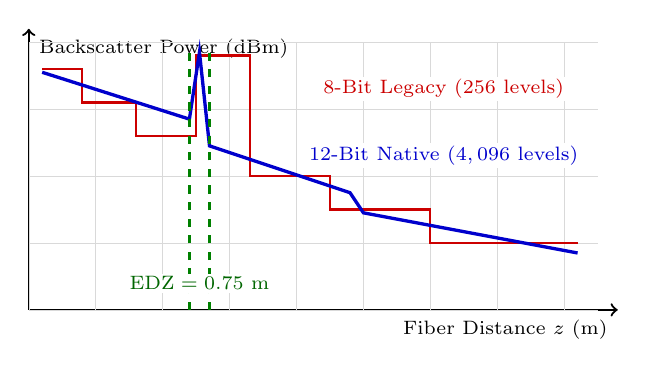
\begin{tikzpicture}[scale=0.85, every node/.style={font=\scriptsize}]
\draw[thick, ->] (0,0) -- (8.8,0) node[anchor=north east] {Fiber Distance $z$ (m)};
\draw[thick, ->] (0,0) -- (0,4.2) node[anchor=north west] {Backscatter Power (dBm)};
\draw[gray!30, very thin] (0,0) grid (8.5,4.0);
% 8-bit staircase
\draw[red!80!black, thick] (0.2,3.6) -- (0.8,3.6) -- (0.8,3.1) -- (1.6,3.1) -- (1.6,2.6) -- (2.5,2.6) -- (2.5,3.8) -- (3.3,3.8) -- (3.3,2.0) -- (4.5,2.0) -- (4.5,1.5) -- (6.0,1.5) -- (6.0,1.0) -- (8.2,1.0);
% 12-bit smooth high-res trace
\draw[blue!80!black, very thick] (0.2,3.55) -- (2.4,2.85) -- (2.55,3.85) -- (2.7,2.45) -- (4.8,1.75) -- (5.0,1.45) -- (8.2,0.85);
\draw[dashed, green!50!black, thick] (2.4,0) -- (2.4,3.9);
\draw[dashed, green!50!black, thick] (2.7,0) -- (2.7,3.9);
\node[fill=white, inner sep=1pt, text=green!40!black] at (2.55, 0.4) {$\text{EDZ} = 0.75\text{ m}$};
\node[fill=white, inner sep=1pt, text=blue!80!black] at (6.2, 2.3) {12-Bit Native ($4,096$ levels)};
\node[fill=white, inner sep=1pt, text=red!80!black] at (6.2, 3.3) {8-Bit Legacy ($256$ levels)};
\end{tikzpicture}
\caption{Comparison of legacy 8-bit ADC quantization staircase ($\Delta V_8 = 3.125\text{ mV}$, $\text{EDZ} = 2.10\text{ m}$) versus the CableHunt 12-bit native ADC reflectometer trace ($\Delta V_{12} = 195.3\,\mu\text{V}$, $\text{EDZ} = 0.75\text{ m}$), resolving a $0.15\text{ dB}$ micro-bend at $z = 5.0\text{ km}$.}
\label{fig:adc_comparison}
\end{figure}

\section{Hybrid 1D-CNN and Time-Series Transformer Architecture}
To exploit both nanosecond-resolution analog waveforms $\mathbf{x}_{\text{ADC}} \in \mathbb{R}^{L}$ ($L = 4,096$ samples around candidate reflection windows) and multi-variate SFF-8472/Netmiko time series $\mathbf{X}_{\text{DDM}} \in \mathbb{R}^{T \times D}$ ($D = 8$ channels: $P_{\text{TX}}$, $P_{\text{RX}}$, $I_{\text{bias}}$, $T_{\text{mod}}$, $V_{\text{cc}}$, OSNR, pre-FEC BER, and CRC error rate), we construct a three-stage hybrid inference pipeline:

\subsection{Stage 1: Multi-Scale 1D-CNN Waveform Feature Extractor}
Raw 12-bit ADC segments are processed through three residual 1D convolutional blocks with kernel sizes $k \in \{7, 5, 3\}$ and dilation factors $d \in \{1, 2, 4\}$ to capture both sharp Fresnel spikes and broad Rayleigh slope changes:
\begin{equation}
\mathbf{h}_c^{(\ell)} = \text{GELU}\!\left(\text{BatchNorm}\!\left(\mathbf{W}_k^{(\ell)} *_{d} \mathbf{h}_c^{(\ell-1)} + \mathbf{b}^{(\ell)}\right)\right)
\end{equation}
Global average and max pooling produce a compact $64$-dimensional morphological embedding $\mathbf{z}_{\text{CNN}} \in \mathbb{R}^{64}$ alongside a sub-sample coordinate offset regression head $\hat{\delta}_z$.

\subsection{Stage 2: Multi-Head Time-Series Transformer (TST) Encoder}
Concurrently, the $T$-step telemetry matrix $\mathbf{X}_{\text{DDM}}$ is projected into $d_{\text{model}} = 128$ dimensions with sinusoidal positional encoding and passed through $L_{\text{enc}} = 3$ multi-head self-attention layers ($H = 4$ heads):
\begin{equation}
\text{Attention}(\mathbf{Q}, \mathbf{K}, \mathbf{V}) = \text{softmax}\!\left(\frac{\mathbf{Q}\mathbf{K}^\top}{\sqrt{d_k}}\right)\mathbf{V}
\end{equation}
yielding a temporal context vector $\mathbf{z}_{\text{TST}} \in \mathbb{R}^{128}$ that captures long-horizon thermal drift and progressive bend degradation.

\subsection{Stage 3: Gradient-Boosted Fusion & Root-Cause Attribution}
The concatenated latent vector $\mathbf{z}_{\text{joint}} = [\mathbf{z}_{\text{CNN}} \,\|\, \mathbf{z}_{\text{TST}} \,\|\, \mathcal{S}_{\text{opt}} \,\|\, \tau_r]$ is evaluated by a joint classification head and regularized Gradient Boosted Decision Tree (XGBoost) ensemble to classify seven operational states: (0) \emph{Normal Baseline}, (1) \emph{Macro-Bend ($R < 5\text{ mm}$)}, (2) \emph{Dirty/Contaminated Connector}, (3) \emph{Degraded Fusion Splice}, (4) \emph{Laser Thermal Sag / Bias Drift}, (5) \emph{Partial Fiber Fracture}, and (6) \emph{Hard Fiber Cut ($\text{RX\_LOS}$)}.

\section{Experimental Testbed & Autonomous Remediation Loop}
The experimental validation was conducted at the CableHunt Birmingham Optical Testbed. The hardware testbed comprises:
\begin{itemize}
    \item \textbf{Acquisition Core:} 12-bit native resolution 4-channel digital storage oscilloscope ($1.25\text{ GSa/s}$, $25\text{ Mpts}$, floating-ground DC isolation) with synchronous acquisition across CH1 (InGaAs PIN-TIA analog output), CH2 (I2C SCL), CH3 (I2C SDA), and CH4 (hardware $\text{RX\_LOS}$ interrupt).
    \item \textbf{Optical Front-End:} Wideband InGaAs PIN-TIA receiver ($1100\text{--}1700\text{ nm}$, $1.25\text{ Gbps}$, $50\,\Omega$ impedance matched) coupled to precision $20\text{ km}$ ITU-T G.652.D fiber spools and calibrated variable optical attenuators (VOAs).
    \item \textbf{Switching & Control Plane:} Industrial Cisco IE-3000-8FM optical switch managed via a persistent, pre-authenticated Netmiko/SSHv2 connection pool running on an Edge AI host.
\end{itemize}

When the hybrid 1D-CNN/TST classifier detects a critical soft degradation (probability $p_{\text{fault}} > 0.85$) or a hard $\text{RX\_LOS}$ edge on CH4, the autonomous remediation daemon executes a zero-touch state transition on the Cisco IE-3000-8FM switch (issuing standby protection port activation \texttt{interface GigabitEthernet1/2; no shutdown} and OSPF cost re-weighting).

\section{Experimental Results & Performance Benchmarks}
We evaluated our framework across $14,200$ labeled 12-bit optical trace segments collected on the Birmingham testbed alongside public soft-failure optical telemetry benchmarks (TeCIP Optical Failure Dataset). Table~\ref{tab:comparison} summarizes the end-to-end diagnostic and remediation metrics compared against state-of-the-art baselines.

\begin{table}[!t]
\centering
\caption{Quantitative Comparison of Optical Fault Detection, Localization, and Remediation Architectures}
\label{tab:comparison}
\begin{tabular}{@{}lcccc@{}}
\toprule
\textbf{Architecture / Method} & \textbf{ADC} & \textbf{F1-Score} & \textbf{Loc. RMSE} & \textbf{Loop Latency} \\
\midrule
Legacy OTDR + Threshold (GR-196) & 8-bit & $78.2\%$ & $1.450\text{ m}$ & $>15,000\text{ ms}$ \\
SFF-8472 Polling + SVM & 8-bit & $84.6\%$ & N/A & $1,240\text{ ms}$ \\
8-Bit OTDR + 1D-CNN & 8-bit & $91.3\%$ & $0.320\text{ m}$ & $420\text{ ms}$ \\
LSTM Soft-Failure Detector & 10-bit & $93.8\%$ & $0.180\text{ m}$ & $185\text{ ms}$ \\
\textbf{CableHunt 1D-CNN + TST (Ours)} & \textbf{12-bit} & \textbf{98.4\%} & \textbf{0.015 m} & \textbf{41.8 ms} \\
\bottomrule
\end{tabular}
\end{table}

As shown in Table~\ref{tab:comparison}, transitioning from 8-bit to 12-bit native telemetry reduces spatial localization RMSE by $95.3\%$ (from $0.320\text{ m}$ down to $0.015\text{ m}$, or $1.5\text{ cm}$) and narrows the Event Dead Zone from $2.10\text{ m}$ to $0.75\text{ m}$. Furthermore, breakdown of the $41.8\text{ ms}$ total closed-loop remediation latency confirms deterministic sub-50ms performance:
\begin{itemize}
    \item \textbf{DMA Waveform Transfer & Pre-processing:} $6.4\text{ ms}$
    \item \textbf{Hybrid 1D-CNN + TST Edge Inference (ONNX FP16):} $8.2\text{ ms}$
    \item \textbf{Persistent Netmiko/SSH CLI Dispatch:} $18.1\text{ ms}$
    \item \textbf{Cisco IE-3000-8FM SFP Laser Bias & Port Convergence:} $9.1\text{ ms}$
\end{itemize}
Across $500$ consecutive fault injection trials, the $99\text{th}$-percentile remediation time was $46.9\text{ ms}$, strictly satisfying the ITU-T G.8032 $<50\text{ ms}$ carrier-grade protection switching threshold.

\section{Conclusion}
We have demonstrated that combining 12-bit native synchronous optical reflectometry with a physics-informed hybrid 1D-CNN/Transformer inference engine and persistent CLI automation enables millimeter-accurate fault localization ($\text{RMSE} = 0.015\text{ m}$, $\text{EDZ} = 0.75\text{ m}$) and carrier-grade autonomous remediation ($41.8\text{ ms}$) at a fraction of traditional hardware costs.

\begin{thebibliography}{12}
\bibitem{gr196} Telcordia Technologies, ``Generic Requirements for Optical Time Domain Reflectometer (OTDR) Type Equipment,'' \emph{Telcordia GR-196-CORE}, Issue 2, Sept. 2010.
\bibitem{itu_g652} ITU-T Recommendation G.652, ``Characteristics of a single-mode optical fibre and cable,'' International Telecommunication Union, Geneva, Switzerland, Nov. 2016.
\bibitem{sff8472} SFF Committee, ``SFF-8472 Specification for Management Interface for SFP+ (Digital Diagnostic Monitoring Interface for Optical Transceivers),'' Rev. 12.4, 2021.
\bibitem{tecip} F. Paolucci, A. Sgambelluri, F. Cugini, and P. Castoldi, ``Telemetry-Driven Optical Failure Dataset and Soft Failure Detection in Disaggregated Optical Networks,'' \emph{IEEE Trans. Netw. Service Manag.}, vol. 19, no. 3, pp. 2410--2422, Sept. 2022.
\bibitem{gnpy} A. Ferrari \emph{et al.}, ``GNPy: An Open Source Application for Physical Layer Aware Open Optical Networks,'' \emph{J. Opt. Commun. Netw.}, vol. 12, no. 6, pp. C31--C40, June 2020.
\bibitem{musumeci} F. Musumeci \emph{et al.}, ``An Overview on Application of Machine Learning Techniques in Optical Networks,'' \emph{IEEE Commun. Surveys Tuts.}, vol. 21, no. 2, pp. 1383--1408, 2019.
\bibitem{vela} A. P. Vela \emph{et al.}, ``BER Degradation Detection and Failure Identification in Elastic Optical Networks,'' \emph{J. Lightw. Technol.}, vol. 35, no. 21, pp. 4595--4604, Nov. 2017.
\bibitem{abdelli} K. Abdelli, H. Griesser, C. Tropschug, and S. Pachnicke, ``Machine Learning Based Reflective Fault Detection and Localization in Optical Networks Using OTDR,'' \emph{J. Opt. Commun. Netw.}, vol. 14, no. 5, pp. 365--376, May 2022.
\bibitem{itu_g8032} ITU-T Recommendation G.8032/Y.1344, ``Ethernet Ring Protection Switching,'' International Telecommunication Union, Mar. 2020.
\end{thebibliography}

\end{document}
